
\documentclass[a4paper, twoside, BCOR20mm, DIV14, headinclude, 11pt, headings=optiontohead]{scrartcl}

\usepackage{lineno}
\linenumbers

\usepackage[pdftex]{graphicx}
\usepackage{epstopdf}
\usepackage[round]{natbib}
%\usepackage{units, calc}
%\usepackage{gensymb} %for \degree and \celsius symbols
%\usepackage[ansinew]{inputenc}
%\usepackage{amssymb}
\usepackage[intlimits]{amsmath} %, fleqn
\usepackage{array}
\usepackage{booktabs}
\usepackage[doublespacing]{setspace}
%\usepackage[font=footnotesize, labelfont=bf, labelsep=endash, labelformat=simple, format= plain, indention=.5cm]{caption}

%required for SI 
%\usepackage{longtable}
%\usepackage{changepage} %for temporal alteration of text width (used in ch1 for table2)

% general settings

%\geometry{verbose, letterpaper, tmargin=2.54cm, bmargin=2.54cm, lmargin=2.54cm, rmargin=2.54cm}

\setcounter{secnumdepth}{0}
\setkomafont{sectioning}{\normalfont\normalcolor\bfseries}
\newcommand*\patchAmsMathEnvironmentForLineno[1]{%
  \expandafter\let\csname old#1\expandafter\endcsname\csname #1\endcsname
  \expandafter\let\csname oldend#1\expandafter\endcsname\csname end#1\endcsname
  \renewenvironment{#1}%
     {\linenomath\csname old#1\endcsname}%
     {\csname oldend#1\endcsname\endlinenomath}}% 
\newcommand*\patchBothAmsMathEnvironmentsForLineno[1]{%
  \patchAmsMathEnvironmentForLineno{#1}%
  \patchAmsMathEnvironmentForLineno{#1*}}%
\AtBeginDocument{%
\patchBothAmsMathEnvironmentsForLineno{equation}%
\patchBothAmsMathEnvironmentsForLineno{align}%
\patchBothAmsMathEnvironmentsForLineno{flalign}%
\patchBothAmsMathEnvironmentsForLineno{alignat}%
\patchBothAmsMathEnvironmentsForLineno{gather}%
\patchBothAmsMathEnvironmentsForLineno{multline}%
}


\begin{document}

%\bibliographystyle{amnat2}


\title{Grazing raises risk of catastrophic shifts in drylands}
\author{Florian D. Schneider \& Sonia K\'efi}
\date{}
\maketitle


\section{Abstract}


\section{Introduction}

Arid rangelands are at high risk of sudden desertification. Overgrazing is considered one of the main causes of desertification worldwide (MEA 2005), an effect which is aggravated by reduced local precipitation and increased temperatures due to global climate change.
The process of persistent vegetation loss under livestock grazing is hardly understood but appear to be  an issue of the system's bistability. Under particular environmental conditions and grazing regimes, two ecosystem states are likewise resilient to perturbations: One state with a robust vegetation cover of shrubs and grasses as well as a desert with no significant vegetation cover (Scheffer 2001, Aguiar and Sala 1999). After crossing critical thresholds, or tipping-points, the system transites between the two stable states.


\begin{figure}[!t]
	\centering
		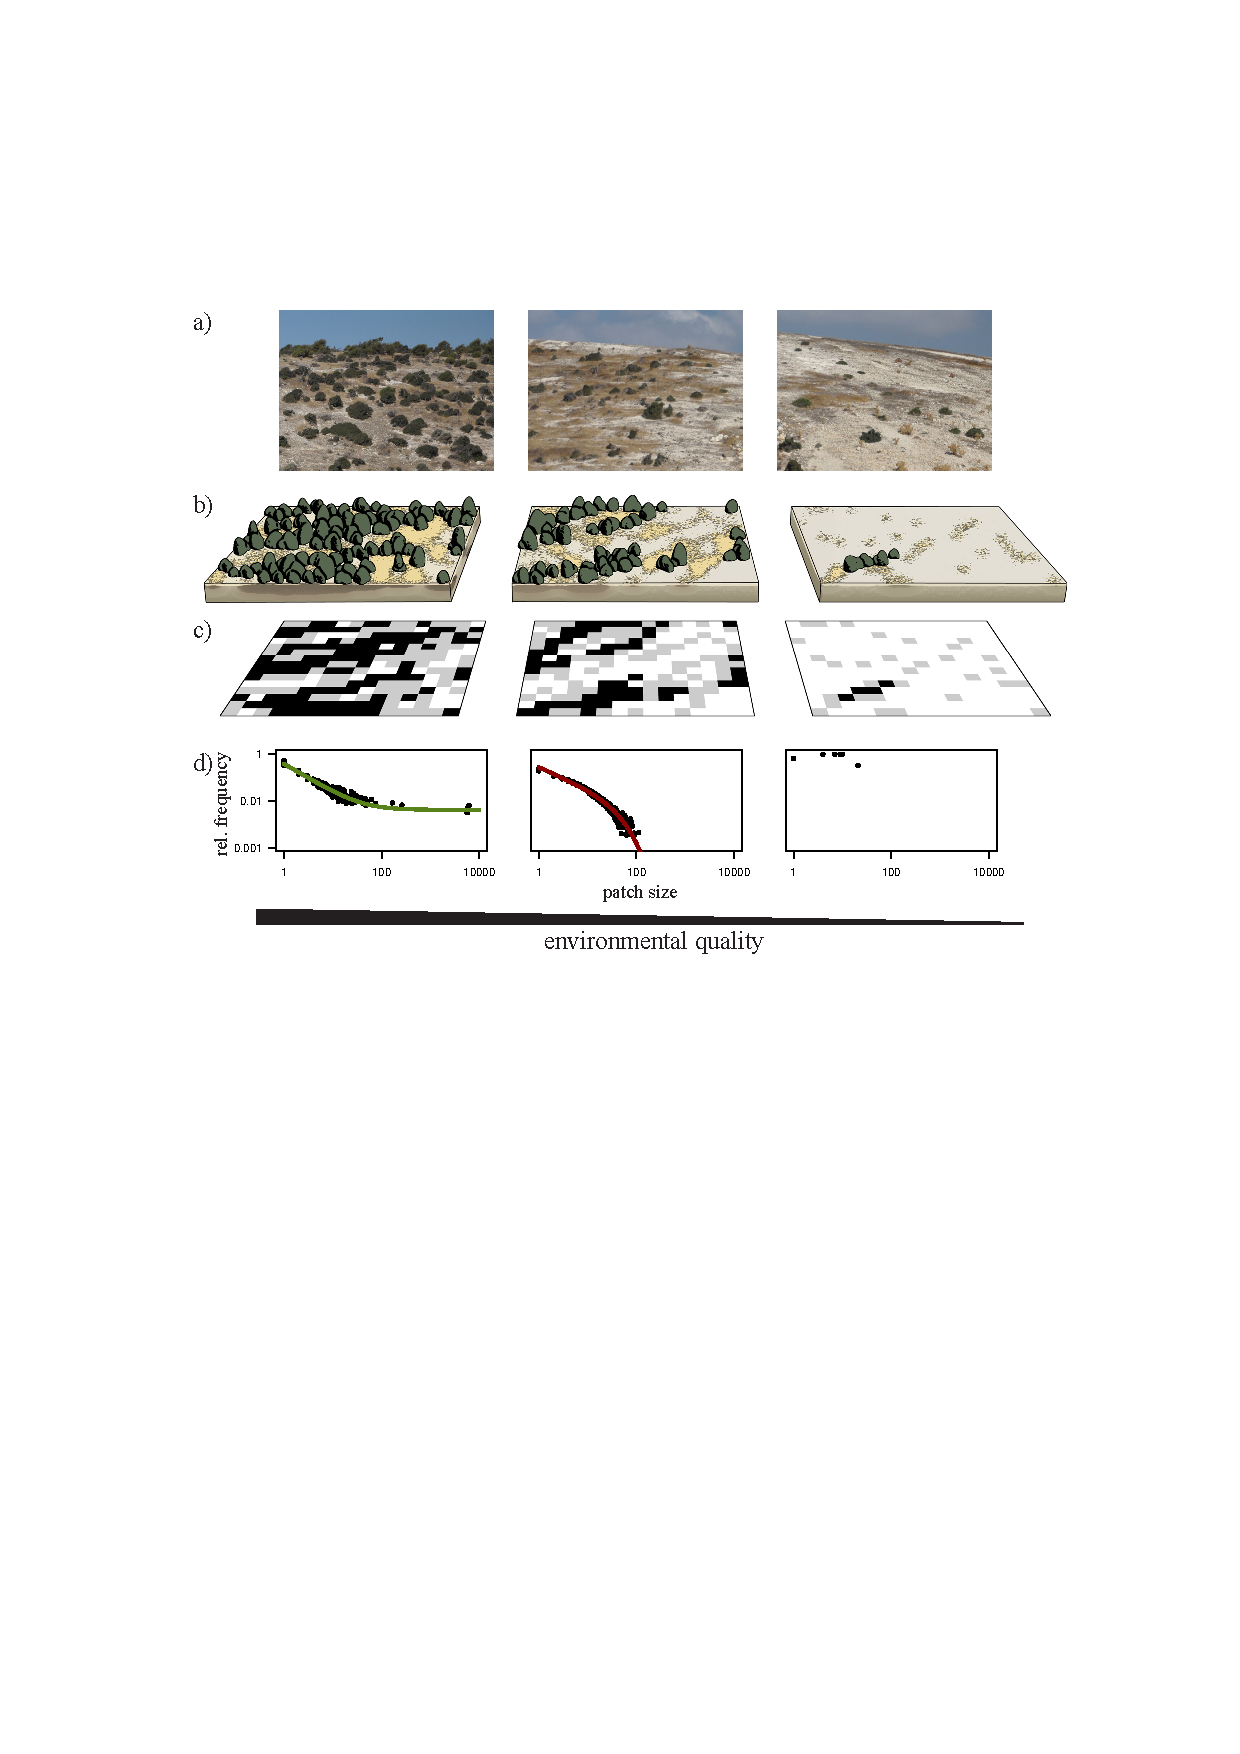
\includegraphics{figures/fig1.pdf}
	\caption{a) Vegetation in arid ecosystems grows in patches. The associated growth provides enhanced local growth conditions as well as protection against grazing. With decreasing environmental quality, vegetation declines and the landscape becomes more fragmented (mid column), leading to desertification (right column). b) Schematic representation of plant patches. The direct neighborhood of plants provides shelter, retention of organic matter and water below and atop the soil surface. Spots remote from vegetation suffer from erosion and evaporation. c) The cellular automata model used in this study therefore distinguishes three states: occupied by vegetation (black), empty but fertile (grey) and degraded (white). d) Cumulative patch size distributions described by power law models: with decreasing environmental quality, the number of large patches declines, turning the power law distribution from up-bent (left) to down-bent (mid). Degraded landscapes have lost all the larger patches and are not to be described by a power law (right). }
	\label{fig:fig1}
\end{figure}


For arid ecosystems, a major mechanism behind this bistability was found to be local facilitation of plant individuals (REF?). The presence of a plant provides its direct local environment with abilities of water retention, organic matter accumulation and protection against external stressors (REF?). Opposingly, spots remote from any vegetation suffer most from erosion and evaporation, leading to locally degraded soils. As a consequence, the vegetation grows in patches (Aguiar and Sala 1999; Fig 1b).  When implemented in a simple spatially explicit model, this positive neighborhood effect provides true bistability on the landscape scale (K\'efi et al 2007a,b; Fig 1c). It therefore can be utilised to investigate the suitability of spatio-temporal metrics to indicate the proximity of a catastrophic shift, such as cumulative patch size distributions or critical slowing down.  

This parent model was used before to investigate the consequences of increased plant mortality (K\'efi et al 2007a). It's simple formulation of additional plant stress can be interpreted as the effects of increased rangeland utilisation, corresponding to the grazing intensity by large herbivores, such as goat and sheep (K\'efi et al 2007a). However, the model has two features that must be considered unrealistic: the individual risk to be harmed by grazing (1) did not vary with total vegetation cover, and (2) it was defined globally and ignored the protective patch structure of the vegetation (Fig. 2a).


\begin{figure}[!tp]
	\centering
		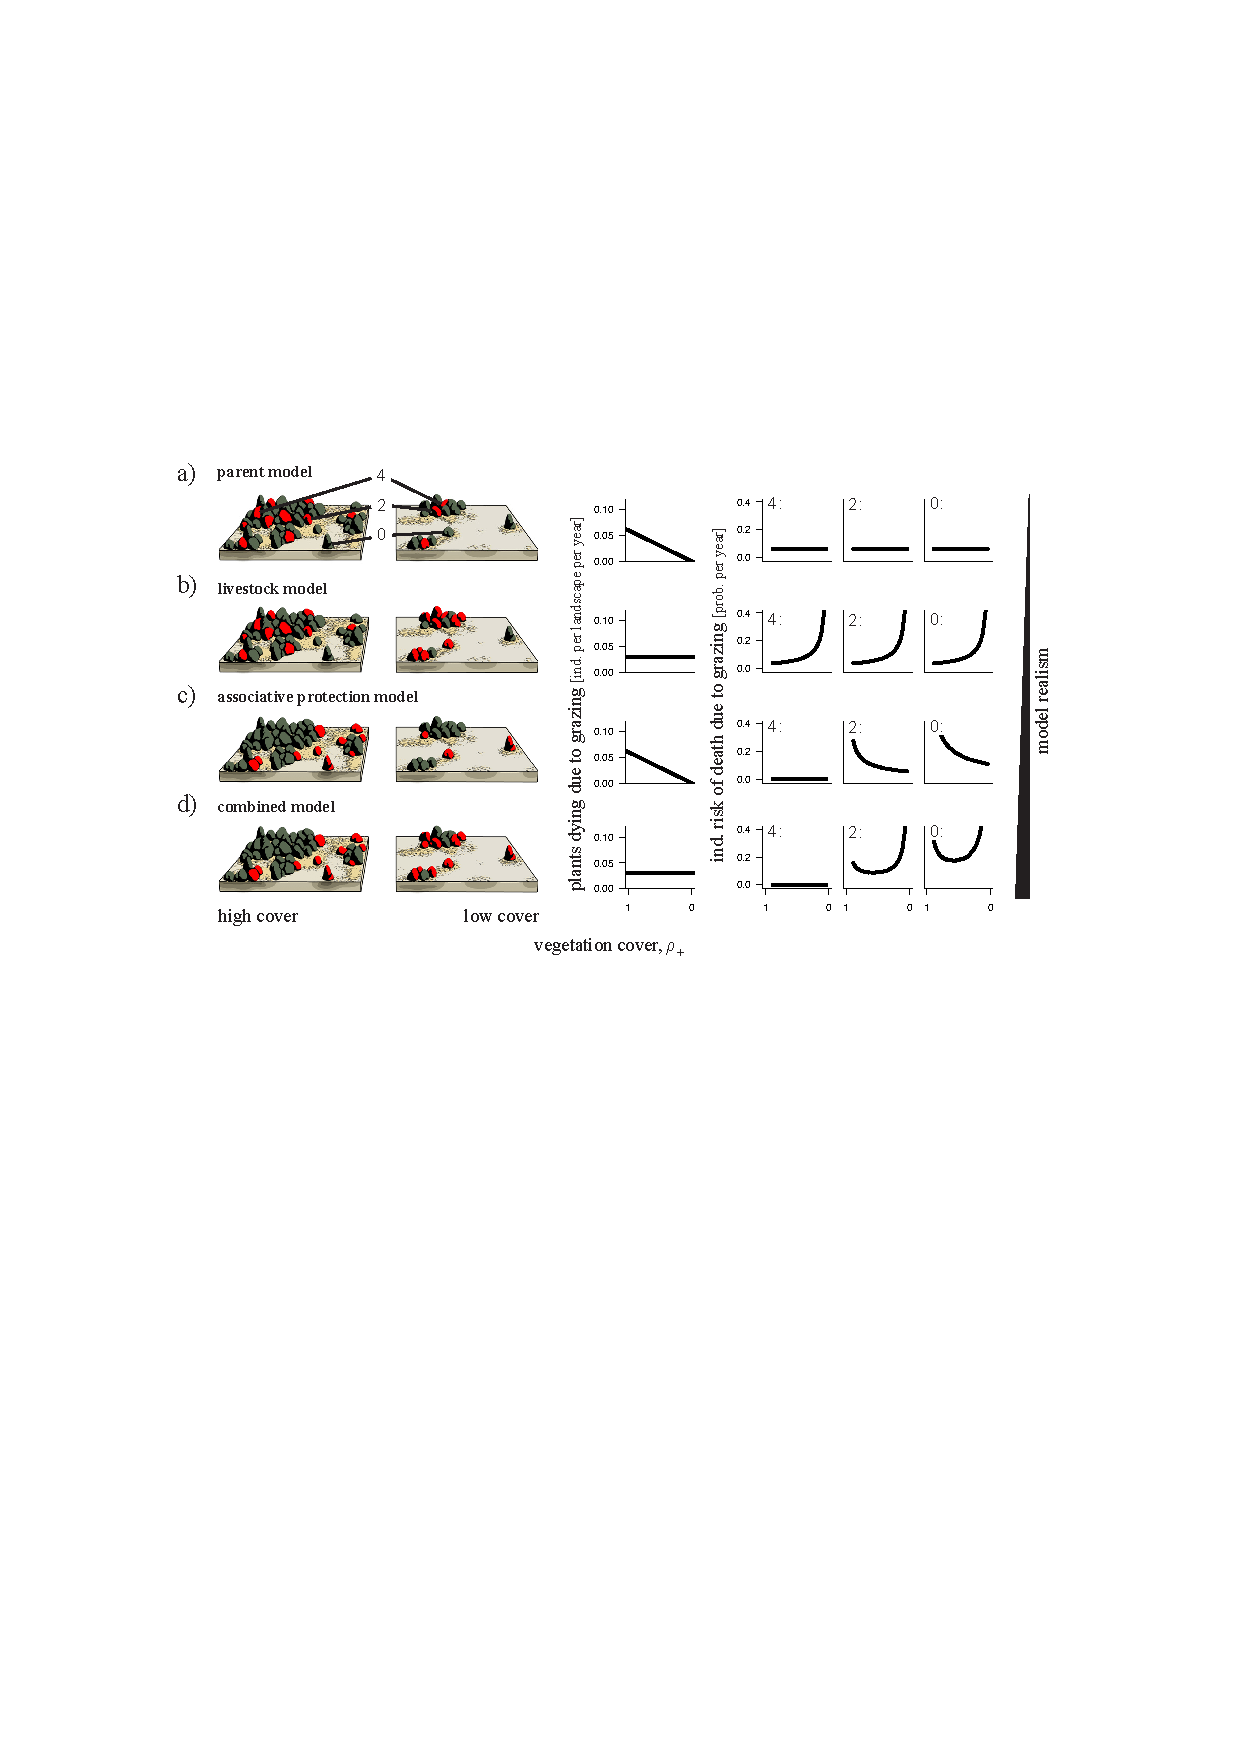
\includegraphics{figures/fig2.pdf}
	\caption{Grazing affects the mortality of individual plants and the patch structure emerging in the landscape. The four models compared in this study use different assumptions on the quantity and spatial differentiation of a particular grazing pressure. Visualized in the left column are the plants dying due to grazing (red). In each model, plants suffer different individual risk, sometimes depending on the number of direct local neighbors (estimates for plants with 4, 2, or 0 neighbors).  a) The \textbf{parent model} as formulated in Kéfi et al 2008 assumes that grazing affects a proportion of living plants, i.e. individual risk is independent of global vegetation cover and shared evenly among all plants. b) The \textbf{livestock model} assumes a constant number of plants dying, regardless of the number of plants available. The individual risk is increasing when vegetation cover is low. c) Assuming \textbf{associative protection} leaves plants in the patch center unaffected by grazing (4), where­as plants at the patch border (2) or growing isolated (0) are suffering more from grazing. Particularly at high vegetation cover, the proportional grazing concentrates on those plants. d) The \textbf{combined model} integrates both assumptions leading to highest individual risk at low and high vegetation cover for isolated plants.  }
	\label{fig:fig2}
\end{figure}

Both assumptions are justified by the need for model simplicity, but disallow a translation of the model parameters to real livestock rates. Increasing individual plant mortality by factor two does not correspond to twice the number of animals per hectar: The proportional character of global plant mortality causes the total pressure on vegetation to decrease when intensive grazing reduces total vegetation cover (Fig 1a).

The relationship between livestock rates and the stability of vegetation cover is a crucial information for management decisions. The present study aims at increasing the realism and applicability of the model by applying two extensions that enable simulations of a grazing gradient on drylands.

%Grazing depends on vegetation cover
The first extension adds a contrasting assumption on the dependence on the total vegetation cover to the parent model. The prior model defined grazing as a constant addition to the risk of a plant to die. On the population level, the number of plants dying because of grazing decreased with a loss in vegetation cover (K\'efi et al. 2007, Fig. 2a). However, grazers forage in the landscape and consume to fulfill their daily demands. In other words, the number of plants suffering from grazing should be rather constant with vegetation cover. As a consequence, at low vegetation cover the grazing risk on individual plants will be high, whereas when vegetation cover is high, risk will be shared among many plants (Fig 2b).
In reality, the total feeding of large herbivores in the landscape is not entirely independent of vegetation cover but follows a non-linear saturating curve (type-II functional response, Holling 1959, Spalinger and Hobbs 1992). Thus, particularly at low vegetation cover, grazing is limited by the search success of the grazer, which is resource-density dependent. In rangeland systems, however, the functional response at low vegetation cover depends on factors on a larger scale: the animals move between landscapes motivated by internal decision patterns or their density is modulated by human management decisions (Senft 1989). We assume therefore, that smooth type-II functional responses, as described for wild ungulates, are unlikely to happen in intensive rangelands within the spatial scale adressed in the present study.

Because of these uncertainties and for reasons of simplicity we contrast the parent assumption of individual plant mortality beeing independent of vegetation cover with a constant amount of global feeding, which results in individual plant mortality increasing with vegetation cover (Fig 2b, right panel). We expect constant global feeding to consolidate both stable states: an almost desertified landscape will be more resilient against recolonisation of single plants while the vegetated state will provide better protection to the plant individual. As a consequence, the reversibility of catastrophic shifts is expected to deteriorate. 

%Spalinger and Hobbs 1992 

%Grazing is spatialy differentiated
The second extension implements a small-scaled, local differentiation of grazing pressure. %For some time, the relationship between vegetation structure and grazing is acknowledged to be interdependent. Grazing affects the mortality of plants as well as plant recruitment, soil suitability, and other factors in positive as well as negative ways. Vegetation cover is a 
%Senft et al 1987
%Bailey 1996
Particularly, the importance of direct neighborhood interactions on the individual plant scale (local scale) in explaining spatial structure was demonstrated by Adler et al. (2001). The authors showed in a theoretical framework similar to the present study, that positive local interactions are superior to environmental heterogeneity or heterogeneous stress in explaining the patterns of plant spatial heterogeneity (Adler et al 2001). 

To differentiate the grazing locally, we implement an associative protection of plant individuals growing next to each other. This mechanism is observed frequently among shrubs in dryland ecosystems and considered to be a major driver of spatial heterogeneity of stress on local scales (REF). 
%Bisigato et al 2005 Ecography
%Milchunas and Noy-Meir 2002
Here, the individual vulnerability against grazing is highest for plants growing isolated. The more direct neighbors a plant associates to, the lower is the effect of grazing. A plant in the patch center is not affected by grazing. We expect this mechanism to benefit the desert state, because at low densities only few plants are associated.

% comparison and main objectives/questions

 We provide a full factorial comparison of the consequences of these alternative models on vegetation structure and the ecosystems' bistability properties.


\section{Methods}
We used a cellular automaton to investigate the consequences of different grazing assumptions on the structural properties of the vegetation. This model was used before (Kefi et al 2007a, b) and can be resolved numerically in spatially explicit simulations. It defines landscape as a grid of cells, each can potentially take one of three discrete cell states: 'vegetated' cells are occupied by a plant individual (annotated as '+' in equations; black cells in figures); 'enriched' cells are suitable for seeds to germinate and colonise the cell, but do not contain adult plants right now  ('0' , grey cells); 'degraded' cells represent bare ground with lacking organic matter and bad water retention, and therefore can not be colonised by arriving seeds  ('$-$', white cells).
Transitions of cells states are only possible between vegetated and enriched (plant death / recolonisation) as well as enriched and degraded (degradation / regeneration). In biological terms, a degraded spot needs to be enriched first, before a plant can grow. Vice versa, when a plant dies, it leaves the spot in an enriched state, which might become degraded later. The rates for these transitions are defined in the following paragraphs. They might be constant values or functions of the global or local plant vegetation density (= $\rho_+$, global vegetation cover; $n_+$) .

\subsection{Facilitation model}
The original model by K\'efi et al mimics local facilitation of plants in drylands by defining the regeneration rate of degraded cells, $w_{ \left\{-,0 \right\} }$, as dependent on the density of vegetated cells in the nearest neighborhood, $\nu_+$ (assessing 'von Neumann'-neighborhood of range 1, i.e. the 4 nearest cells, $\nu_+ \in \left\{ 0, 0.25, 0.5, 0.75, 1 \right\}; $ K\'efi et al 2007b).
\begin{equation}
	w_{ \left\{-,0 \right\} } = r + \nu_{+} f
\end{equation}
% this is defining the rates of change of the population of cells in state '-'. 
%express rates rather as "probability of cell i,j to change into state x given that it is in state y".
The recolonisation of enriched cells takes into account that the majority of seeds arriving on a cell are from the plants in the direct neighborhood (local seed dispersal), while the probability of a successful plant establishment is limited by the competition on global resources.
\begin{equation}
	w_{ \left\{0,+ \right\} } = \left( \delta\rho_+ + \left( 1 - \delta \right)q_{+|0}\right) \left(b-c\rho_+ \right)
\end{equation}

%detailled description of parameters
The degradation of enriched cells is defined as a constant rate	
\begin{equation}
w_{ \left\{0,- \right\} } = d.
\label{eq:}
\end{equation}
Finally, in the original model, the intrinsic mortality of vegetated cells also is defined as constant $w_{ \left\{+,0 \right\} } = m$. Since it is defined as the probability of plant death per year, it also can be interpreted as inverse of the average lifespan of plants. However, the authors assume that this mortality might be increased by external stressors such as grazing. In the following paragraph, we explore different assumptions on how grazing affects the mortality of plant individuals.

\subsection{Grazer Models}
The \textbf{parent model} was used to explore consequences of increased plant mortality due to grazing. It simply adds grazing as a constant to individual mortality rate, affecting all plants homogenously.
\begin{equation}
	w_{ \left\{ +,0 \right\} }  = m_0 + g
\end{equation}
Therefore, $g$ . 

On the landscape scale, this means that vegetation loss due to grazing scales linearly with plant vegetation cover (Fig. 1a). However, while some stressors might change the intrinsic mortality of all plant individuals, independendly of the vegetation cover (e.g. fungal pests, drought), this is certainly not true for grazing.

Instead, in reality the impact of grazers varies strongly with plant vegetation cover. In the \textbf{livestock model}, we approximate the behaviourial responses of grazers to vegetation cover by the following assumption: The number of plants dying due to grazing should correspond to the biomass consumed by a number of grazers in the landscape, while being independent from vegetation cover  (Fig. 1b). Thus, individual risk is high, when few plants are present in the landscape and it is low for high vegetation cover. The correlation between vegetation density and individual risk is as follows. 
\begin{equation}
	w_{ \left\{ +,0 \right\} }  = m_0 + g_0 / \rho_+
\end{equation}
The two models therefore produce differing mortalities in cases departing from  $ \rho_+ = g_0 / g$. For densities $ \rho_+ < g_0 / g$, the livestock model produces higher mortality than the parent model. For $ \rho_+ > g_0 / g$, the opposite is the case. Since density is dynamic over time, with attractors depending on total individual ... 

To compare the two models, we define them to have equal mortality at intermediate vegetation cover, $\rho_+ = 0.5$. Therefore, in the parent model $g$ is set to be $g_0/0.5$. 

\subsection{Associative Protection}
Plants benefit from associative growth in an environment with physical stressors like grazing. Shrubs in particular shield each other from grazers when growing in direct neighborhood. Therefore plants growing isolated suffer more from grazing than plants growing within patches.
The models from the previous paragraph do not account for this locally differentiated impacts of grazing. To add \textbf{associative protection} to the model we need to define individual vulnerability, 
\begin{equation}
v = 1 - \nu_+ ,
\end{equation}
to decrease with the density of vegetated neighboring cells $\nu_+$. It is highest for isolated plants with no neighbors ($\nu_+ = 0$) and decreases linearly with the density of vegetated neighboring cells. A plant with four vegetated neighbors ($\nu_+ = 1$) is not vulnerable to grazing. 
To keep global grazing in accord to the parent model or the livestock model we normalize vulnerability against the average vulnerability of all vegetated cells,

\begin{equation}
\widehat{v} =  \frac{ \sum\limits_i{ 1 - {\nu_+i}}  } {n_+} ,
\label{eq:vul}
\end{equation}
yielding
\begin{equation}
	w_{ \left\{ +,0 \right\} }  = m_0 + g_0 / \rho_+ \frac{v}{\widehat{v}}.
\label{eq:}
\end{equation}

Therefore, we compare two spatial variants of grazing (spatially homogenous \textit{vs.} associative protection) for each grazer model (parent model with constant risk \textit{vs.} lifestock model with density dependent risk; see Table 1). 



\begin{table}[!th]
\label{tab:models}
\caption{the models' substitutions for grazing,  $g$, in the mortality term $w_{ \left\{ +,0 \right\} }  = m_0 + g$.  }
\centering
\begin{tabular}{ccc}

\toprule
 & parent model & lifestock model \\ \cmidrule(rl){2-2} \cmidrule(rl){3-3}
homogenous grazing &  $g_0/0.5$ & $g_0/\rho_+$\\
associative protection & $g_0/0.5 \frac{v}{\hat{v}}$  & $g_0/\rho_+ \frac{v}{\hat{v}}$ \\
	\bottomrule
\multicolumn{3}{p{9.5cm}}{\footnotesize $m_0$ : intrinsic mortality rate of vegetation, i.e. inverse of average lifespan, $g_0$: grazing intensity, $\rho_+$ : vegetation cover , $v$ : vulnerability, $\hat{v}$: mean vulnerability of all vegetated cells }
	\end{tabular}
\end{table}
%$n_+$ : number of vegetated cells on the lattice \par
%$\rho_+$ : global density of vegetated cells \par
%$\nu_n$ : density of neighbors in state n \par
%$g$ : grazing pressure



\subsection{Numerical simulations}

We applied these rules on a grid of 100 $\times$ 100 cells of 0.25m$^2$. Each timestep is defined as one year. The applicable transition probabilities for each single cell given in equations 1, 2, 3 and 4 are compared against uniform random numbers between 0 and 1 to determine if a transition occurs or if the cell remains unchanged. To initialize the grid with a standardized patchy vegetation structure, each model simulation was run for 500 years without any grazing (g = 0) using an initial environmental value $ b_ini \in \left\{ 0.25, 3, 0.8, 0.9 \right\} $ before grazing is taking action. %(Note: I want to complete this to a highly resoluted gradient, to investigate the unstable equilibria). 
Starting from the preconditioned grids, the four grazing models (Table 1) with varying grazing intensity ($ g \in \left\{ 0, 0.025, 0.05, 0.075, 0.10 \right\} $) were run over a gradient of environmental quality ($ b \in \left\{ 0.2, ... , 1.0 \right\} $) for 1.500 timesteps. 

An average vegetation cover, $\rho_+$, as well as the average cell mortality,$\hat{m}$ , is determined as the average density of all grids of the final 500 timesteps.


\subsection{Choice of parameters}

To investigate the bistability properties of the vegetation cover, we simulate a high resolution gradient in environmental quality $b$ ranging from 0.2 to 1 with varying step-width between 0.0025 and 0.025. The models of this study inherit all parameters from the parent model in K\'efi et al. 2007a ($r = 0.01$, $f = 0.9$, $\delta = 0.1$, $c = 0.2$, $d = 0.1$), while substituting mortality with Eq. 4 and Table 1. We assume intrinsic mortality $m_0$ for all models to be 0.05, reflecting an average individual lifespan of 20 years, if no additional mortality due to grazing is taking effect.  
Further, we run all models over a linear grazing gradient with $g$ taking 0, 0.025, 0.050, 0.075, 0.100.
For the parent model, this produces average individual lifespans of 20.0, 13.3, 10.0, 8.0, 6.7 years, respectively. 

\subsection{Cumulative patch--size distributions}
We investigate qualitatively, how the patch size distributions change with environmental quality at the different levels of grazing. Therefore, we assigned each simulation run to one of the following five cases: (1) fully vegetated, if the vegetation cover was significant (\> 2 \% ) and aggregated into one large spanning cluster (ignoring additional patches up to a size of 2 cells); (2) up-bent power law, if the cumulative patch--size distribution was best described by a power law with a lower limit defined by a single large spanning cluster; (3) power law, if the cumulative patch--size distribution  was best described by a power-law; (4) down-bent power law, if the cumulative patch--size distribution was best described by a truncated power law; (5) degraded, if the vegetation cover was insignificant (\< 2\%).

We compare the parameter space occupied by those cases. Additionally, we compare the exponent of the power law for the cases 2--4. 

\section{Results}

\newpage

\begin{figure}[h]%
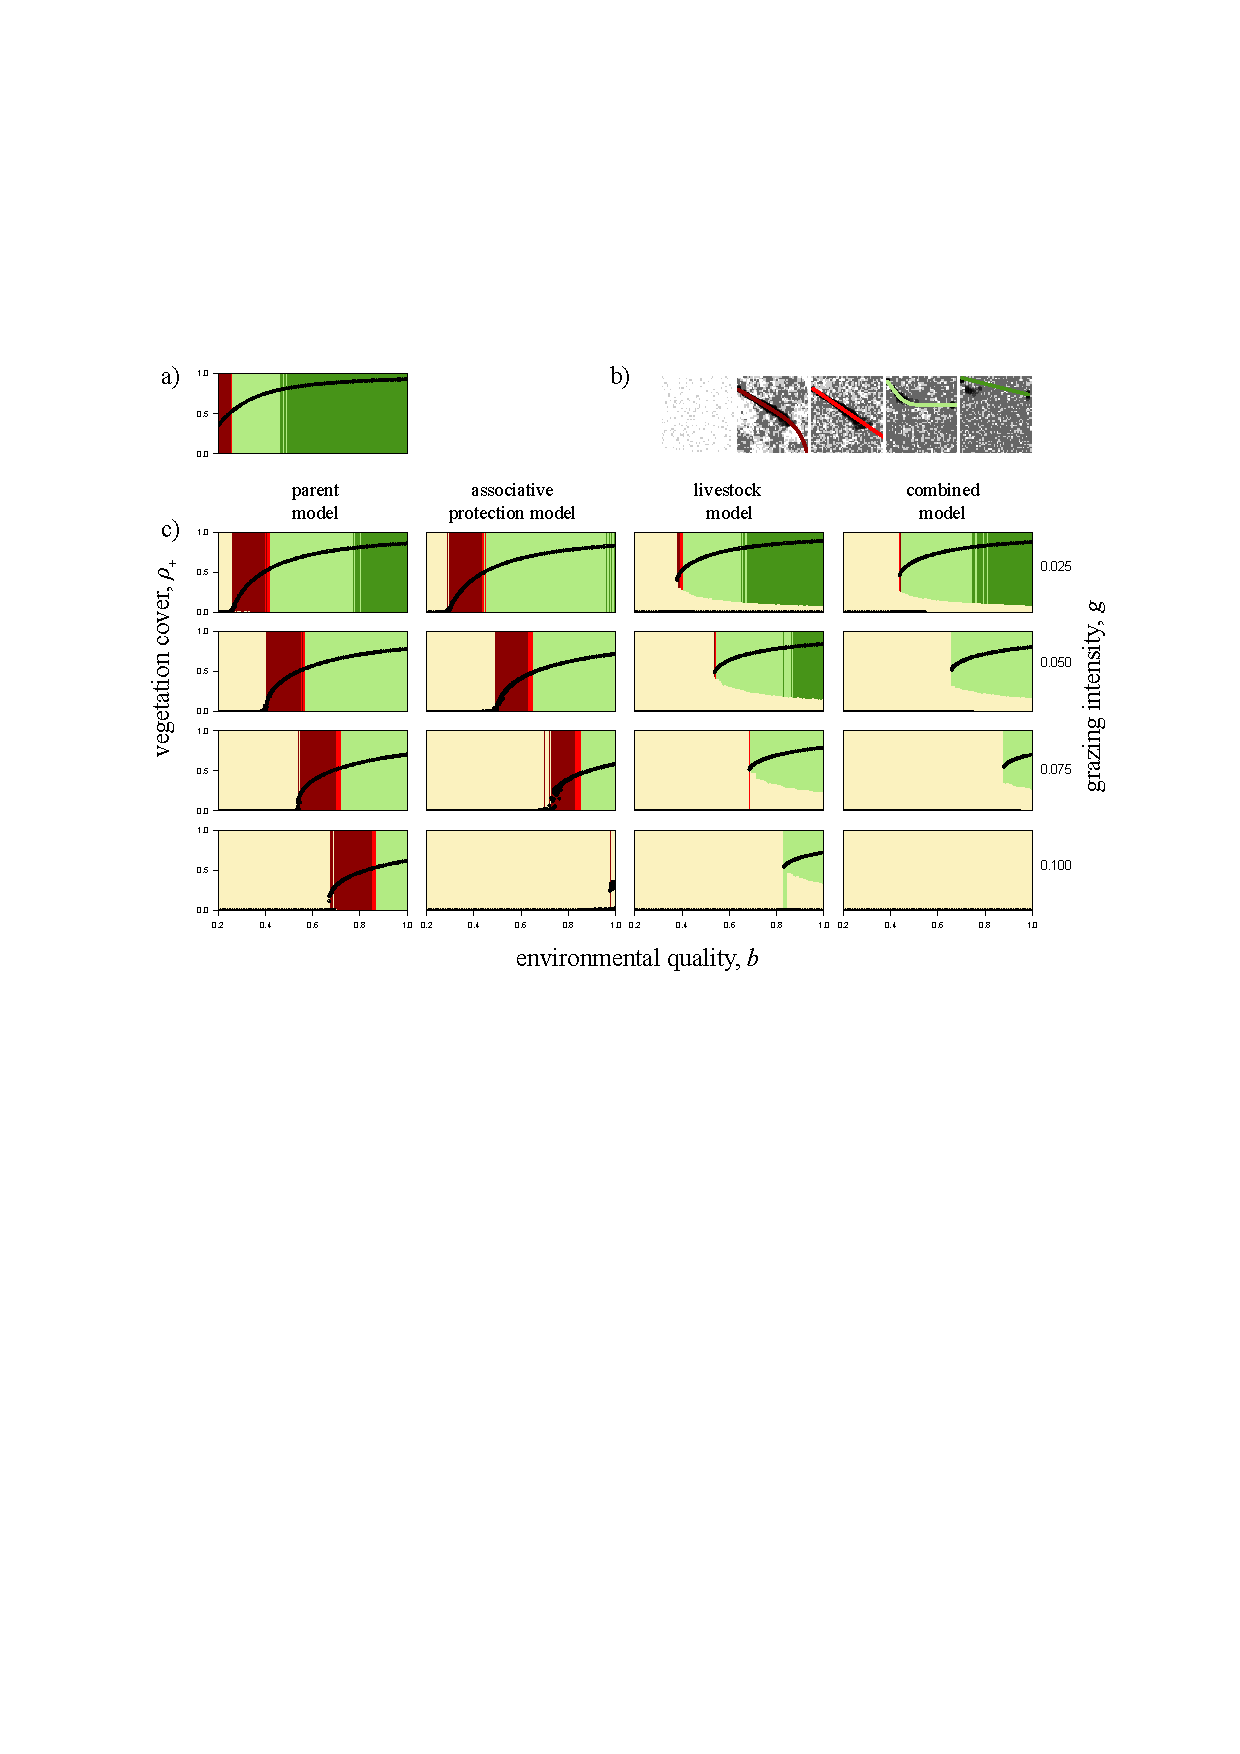
\includegraphics[width=\columnwidth]{figures/fig3.pdf}%
\caption{}%
\label{}%
\end{figure}


\begin{figure}[h]%
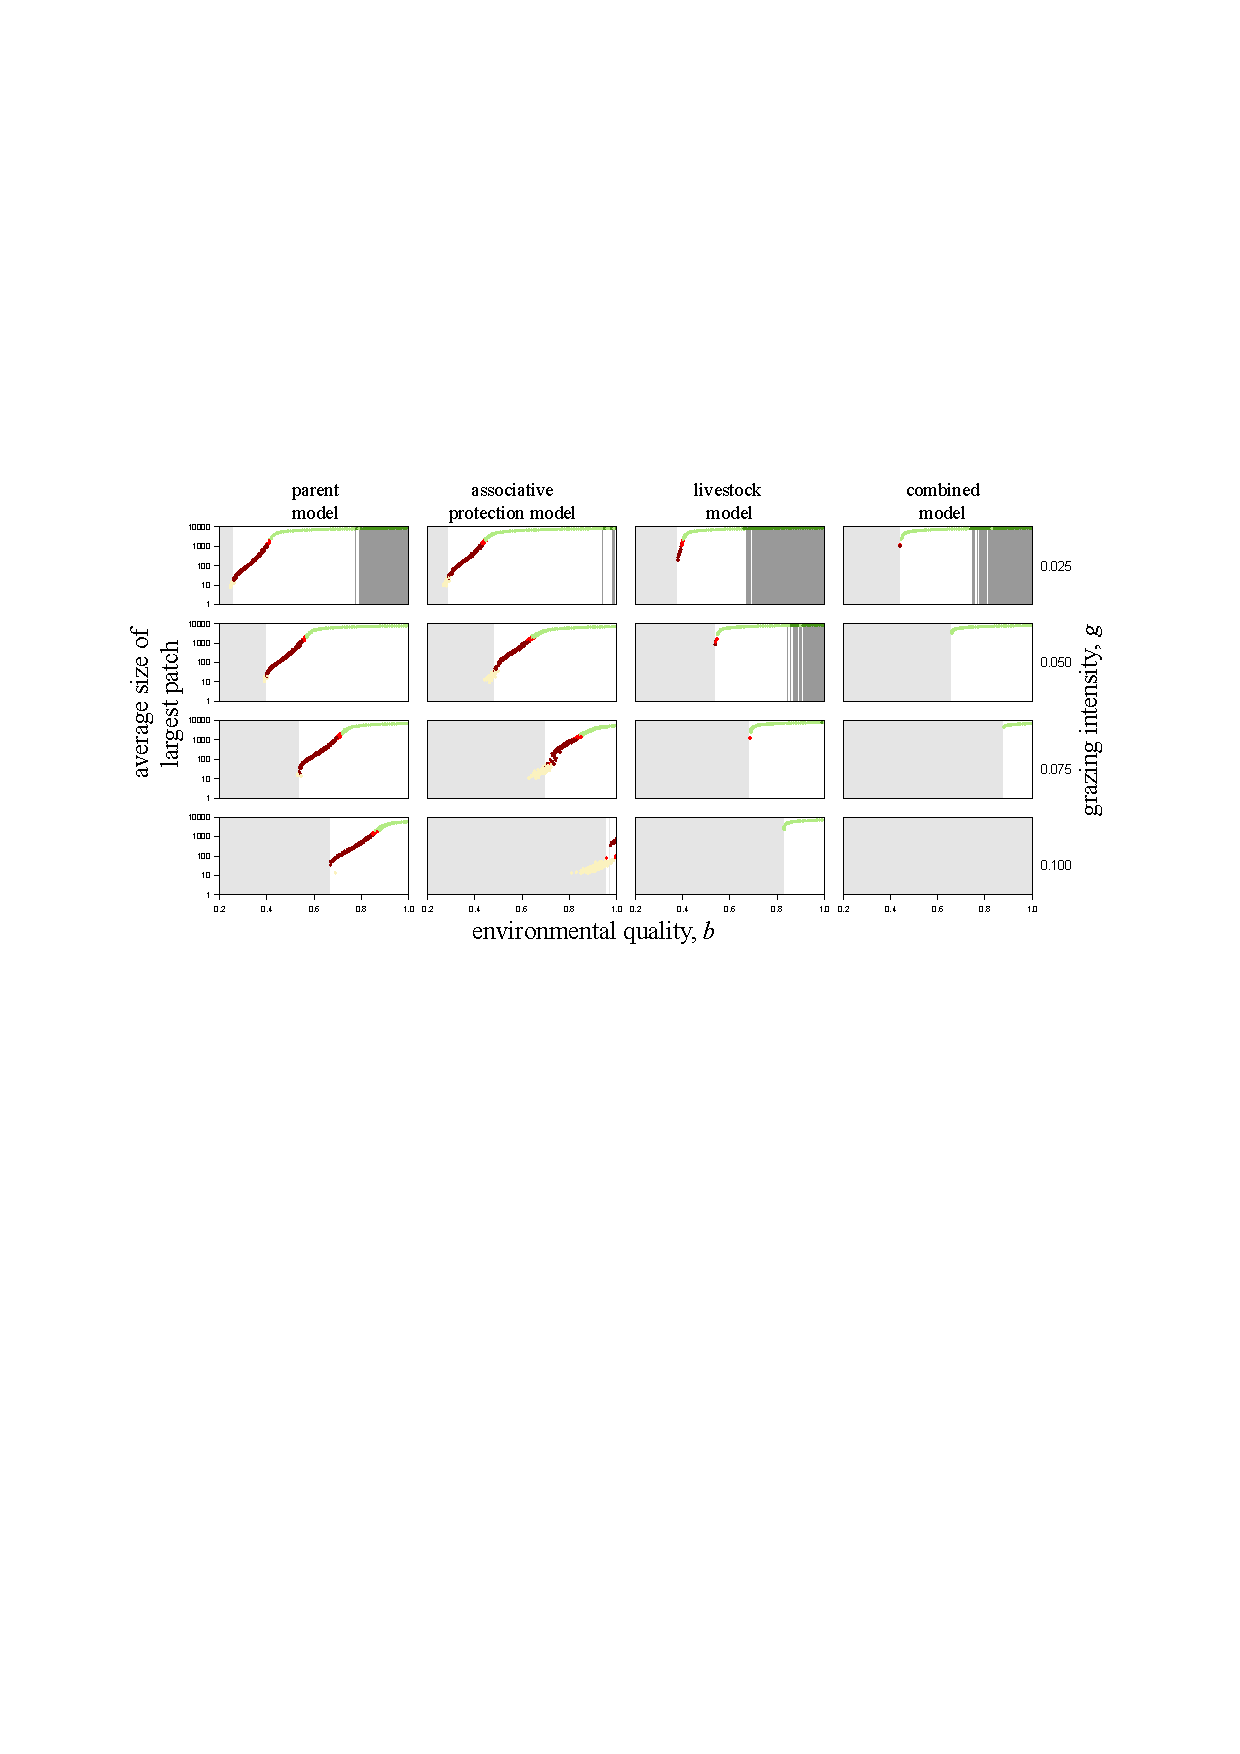
\includegraphics[width=\columnwidth]{figures/fig4.pdf}%
\caption{}%
\label{}%
\end{figure}

\begin{figure}[h]%
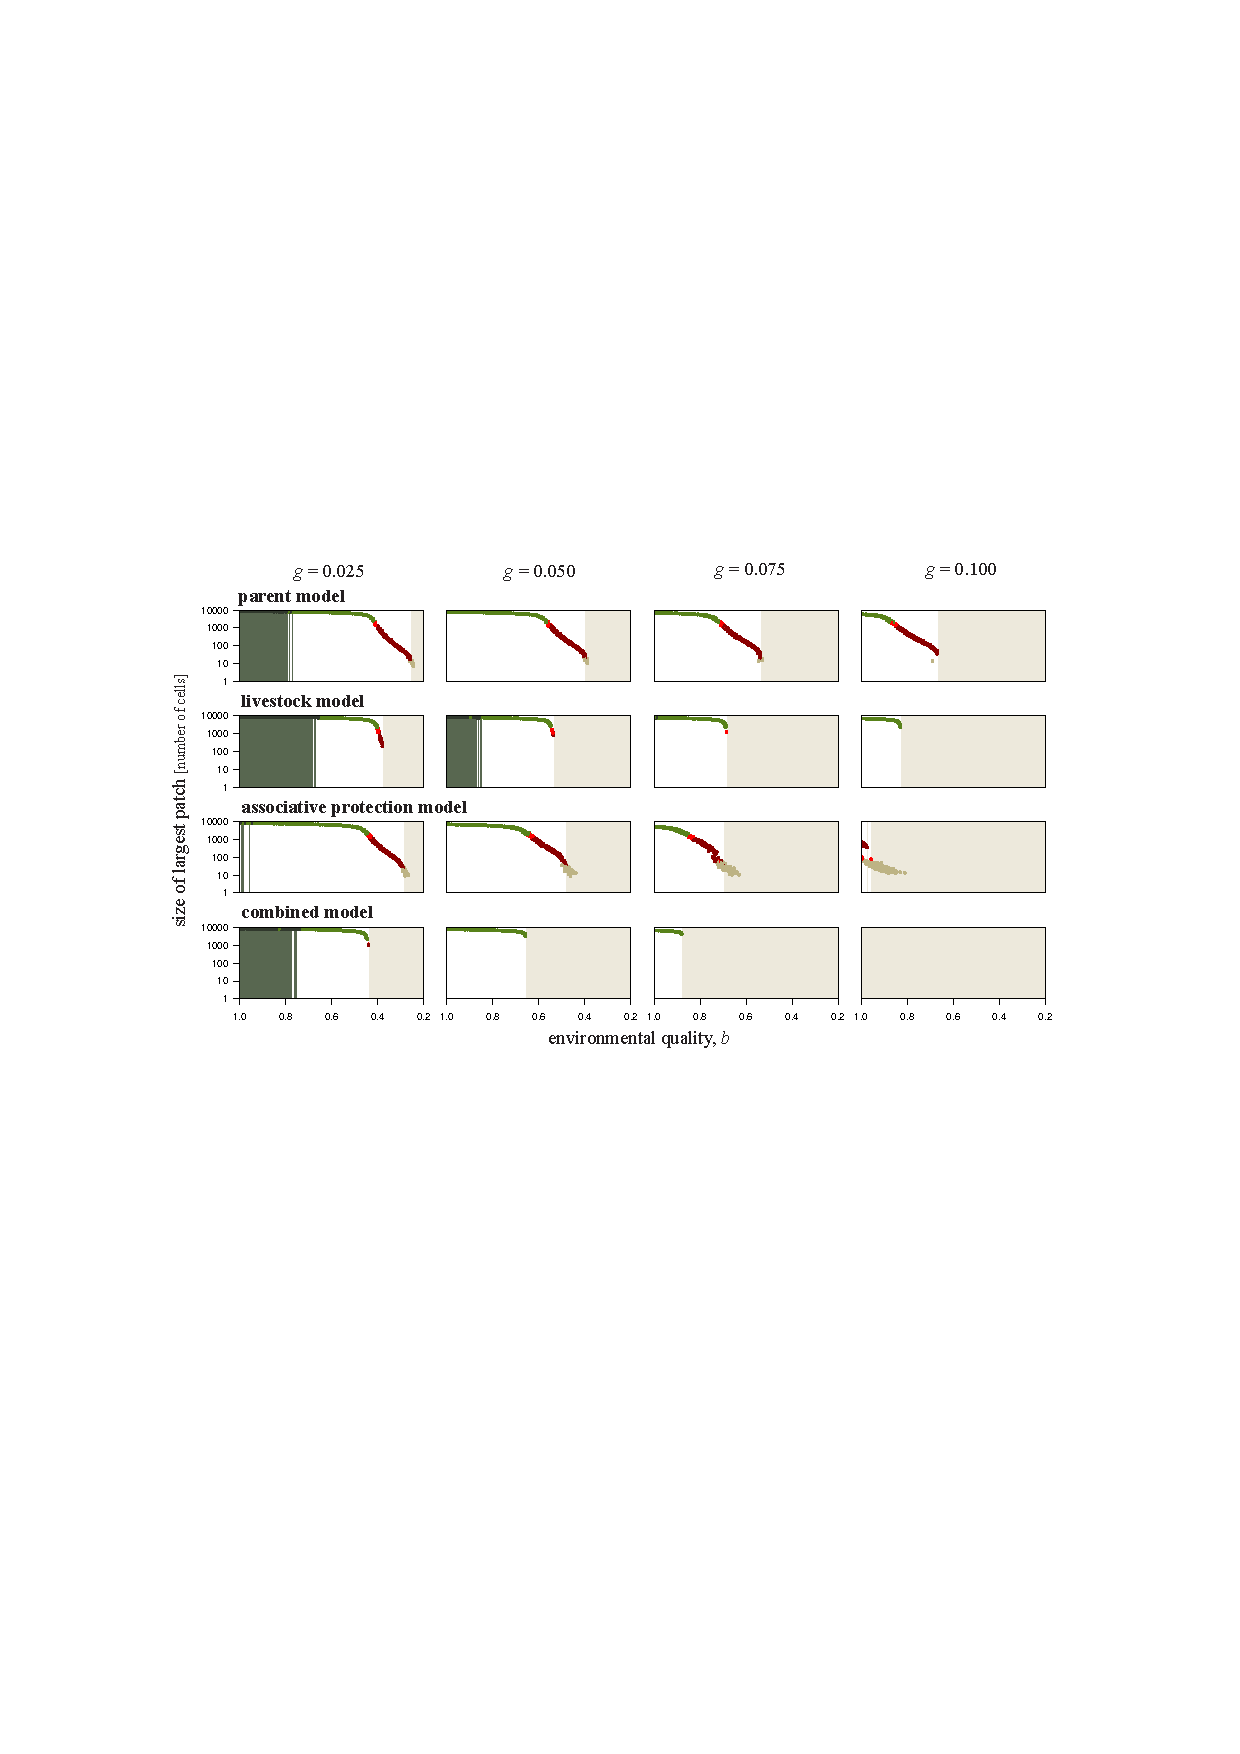
\includegraphics[width=\columnwidth]{figures/fig5.pdf}%
\caption{}%
\label{}%
\end{figure}



\section{Discussion}

Caveats
Functional response of large herbivores; Individual based, informed foraging


In reality, however, the functional response of large grazers on vegetation, particularly at low vegetation cover, is dynamic. In rangelands, management decisions and spatial responses of the grazers will reduce feeding pressure at very low densities. 

In fact, the local effects of large herbivores on plants are manifold and qualitatively different. While direct feeding reduces biomass in the first place, it might lead to growth enhancement and increased productivity. On the local scale, vegetation benefit from the presence of herbivores through fertilization, inoculation with seeds, 
In our model, however, we simplify these factors to a linear negative impact of grazer presence on the local vegetation. The  

\section{Conclusion}
Undifferentiated model underestimates consequences of grazing with regard to the stability properties of the landscape. 
A linear increase in grazing causes shifts much  

\section{APPENDIX}

\subsection{simulations}

The grid was defined to have periodic borders, connecting the east border to the west, the north to the south.
Prerun for 100 years. 
during pre-run, environmental conditions $b_ini \in \left\{ 0.250, 0.274, 0.300, 0.329, 0.360, 0.395, 0.433, 0.474, 0.520, 0.570, 0.624, 0.684, 0.749, 0.821, 0.900 \right\} $ emerge a patch structure ranging from low to high vegetation cover. Trajectories towards a stable vegetated state or towards desert are documented and used to approximate the unstable equilibrium.

, the whole grid is updated synchronously multiple times, to increase stochasticity
each time step is devided by the number of updates per year ( = 5) and

\subsection{model fitting}
 Four models were compared on each snapshot of t


\begin{table}[t!]
\label{tab:fitmodels}
\caption{ Models describing patch size distribution }
\centering
\begin{tabular}{lll}

\toprule
 & function & log-transform \\ \cmidrule(rl){2-2} \cmidrule(rl){3-3}
Power Law &  $n = a s^{- \alpha}$ & $ \log{n} =\log{a} - \alpha \log s$\\
Limited Power Law &  $n = b + a s^{- \alpha} $ & $ \log{n} = \log a - \alpha \log{s} + \log(1+\frac{b}{a s^{-\alpha} })$\\
Truncated Power Law & $n = a s^{- \alpha} \mathrm{e}^{s \frac{1}{S_x}}$  & $\log{n} = \log a  - \alpha  \log s  - s \frac{1}{Sx}  $ \\
%Exponential &  $n = a \mathrm{e}^{-\varepsilon s} $ & $ \log{n} =  \log{a} - \varepsilon s $\\
	\bottomrule
\multicolumn{3}{p{12.5cm}}{\footnotesize  }
	\end{tabular}
\end{table}


table with log-transformed models


 

%\bibliography{biblio}

\end{document}